
%************************************************
\chapter{General discussion and conclusions}\label{ch:discussion}
%************************************************

\tikz[remember picture,overlay] \node[opacity=0.3,inner sep=0pt] at (current page.center){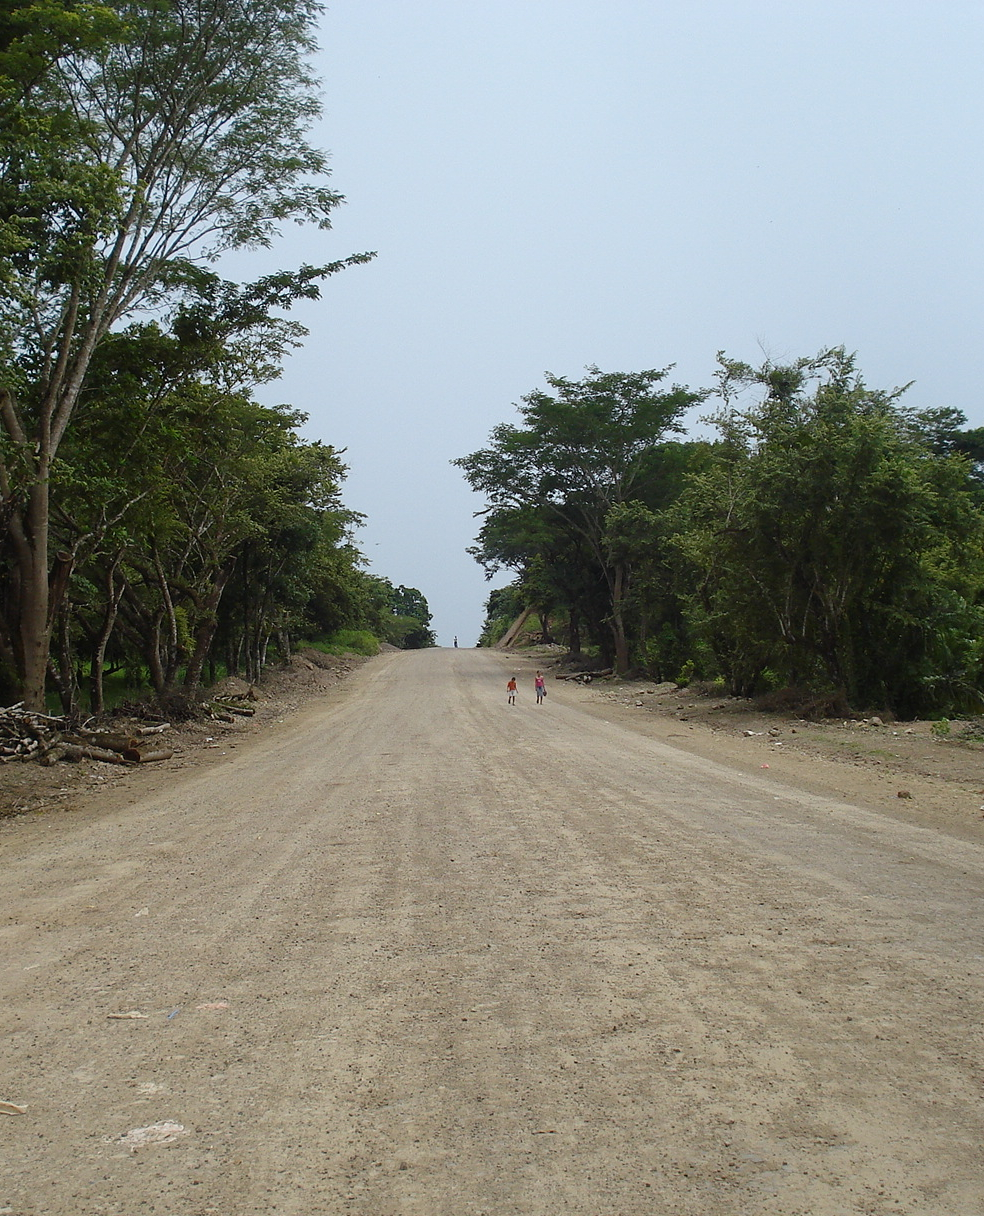
\includegraphics[width=\paperwidth,height=\paperheight]{./Figures/cover/carretera_nica_pagina.jpg}};
\clearpage

We live in a time in which global environmental changes are occurring at unprecedented scales and speeds \citep{Pachauri2015}. Individual species and whole ecological assemblages face systemic risks from a variety of stressors, including the loss and fragmentation of suitable habitat, alterations in the temperature and precipitation regimes, pollution, or an increase in the rate of colonization of human-borne potentially invasive species \citep{Vitousek1994}. Given the scale and magnitude of the human alteration of the environment, it is urgent to develop mitigating measures at all levels, from actions in local habitats to coordinated worldwide socioeconomic efforts that bring us closer to a harmonious coexistence with the non-human world. In order to move towards this admittedly utopian objective, we need the strongest possible scientific understanding of how ecological species and communities are structured, and how they function. In a testimony to the complexity of the natural world, our knowledge of ecological communities is still limited, despite decades of continued work by generations of naturalists and ecologists. In particular, we do not know whether pairwise interactions between individuals are structured in order to enhance community stability sensu lato. When certain interactions are considered in isolation, e.g. trophic or mutualistic ones, theoretical \citep{Williams2000} and empirical \citep{Thebault2010} studies have shown that interactions are indeed distributed non-randomly. However, species in ecological communities display a wide array of interaction types and mechanisms, and we are only starting to gain a broad understanding of how the different interactions combine in natural systems \citep{Kefi2015}, and its implications for ecological processes \citep{Pocock2012}.

In this thesis, I have explored several fundamental questions about networks of ecological interactions, their structure and dynamics in different contexts. In the following paragraphs, I discuss some of the main findings of the thesis and potential lines of work arising from them, in light of the current literature knowledge.

There are only a handful of empirical datasets that account for multiple interaction types in ecological communities (chapter 2). It is therefore only logical that most studies that analyse these complex networks are theoretical in nature, but even restricting ourselves to theoretical models for building and analyzing multiple interactions networks, the diversity of approaches and objectives is already substantial. I have shown that, on a conceptual level, this diversity of modelling strategies boils down to three types of approaches (chapter 2). This conceptualization may help researchers design theoretical studies with a clearer understanding of the limitations and strengths of the methodologies used. For example, not all interaction types occur in the same spatial and temporal scales. Models that lump together interaction effects in a single parameter and do not differentiate spatiotemporal patterns (such as the model developed in chapter 3) should be very explicit about these limitations, and in any case, should be considered baseline models, potentially useful for (1) guide further, more targeted theoretical and empirical work, and (2) comparison against more realistic models. Looking at the broad picture, one may ask whether the increase in model complexity and data collection programs necessary for accounting for different interaction types is worth it, i.e. if it significantly improves our understanding of ecological communities. Although the field is still young, and all conclusions are based on highly idealized models or on very specific, likely incomplete datasets, current results suggest that, indeed, integrating the variety of interactions present in nature into the study of ecological networks produces novel insights and unexpected outcomes, regarding for example the patterns of secondary extinctions in networks \citep{Pocock2012,Evans2013a}, the functional groupings in communities \citep{Kefi2016a}, or, as shown in chapter 3, the persistence of species in their local communities. It remains to be seen, however, if a truly consistent program of data collection across different community types and environmental gradients is feasible, or how more modest experiments such as microcosms can be designed for taking full advantage of this view of ecological communities.

As stated above, before we can extract robust conclusions from empirical data, we may advance our understanding of multiple interaction networks by developing general, overarching models and theories. With that objective in mind, I developed the model of chapter 3, and in its design, I brought together a series of separate insights about interaction networks. In particular, the way in which interactions are quantified is based on the assumption that the abundance of the interacting species is related to their interaction frequency: the more abundant the two species are, the more will they interact. Interaction frequency is, in turn, taken as a measure of the impact of one species over another. This assumption has been corroborated for a number of plant-pollination networks \citep{Vazquez2005,Vazquez2007,Vazquez2012}, but it probably does not hold generally for all interaction types, and it explicitly neglects specialization in ecological interactions. Nevertheless, it represents a robust approach for integrating with a single currency the effects of disparate interaction types in dynamic models.

The results from chapter 3 open different avenues for future research. The most straightforward extension would be the development of experimental or observational studies for testing some of the results: in particular, it would be feasible to test whether species-poor communities tend to have a higher prevalence of positive interactions, as suggested by our theoretical results, and how are these interactions distributed. The assumption that interactions are distributed non-randomly proved key for maintaining high levels of persistence: even in species-poor communities, interactions should maintain a certain structure. Such targeted empirical work could also start to unveil the frequency and structure of less studied interactions. Amensalism and commensalism have been shown in another recent study to improve community stability when accounted for \citep{Mougi2016a}, but they are clearly underrepresented in the literature. Another theoretical outcome from that chapter that would require further study is the observed relationship between the frequency of occurrence of the different interaction types and their connectance values (Appendix 3.4). As long as the set of feasible potential links varies for the different types of interaction, frequency of occurrence and connectance will not be equivalent. I believe that the calculation of connectance relative to fully connected networks should be approached with caution, as there are countless examples in which many of the potential interactions are forbidden because of, for example, non-overlapping activity in time or space \citep{Yang2010,Osorio2018}. In any case, it is unlikely that in multitrophic networks, the set of, say, potential mutualisms, would be the whole network. When evaluating more thoroughly structural metrics of multiple interactions networks, these details should not be overlooked. Note that, throughout chapter 3, I have purposely concentrated on species abundances and already established interactions. Trait-based approaches for inferring interactions \citep{Morales-Castilla2015, Bartomeus2016} and community structure \citep{Laigle2018} also show great promise, but they are difficult to generalize to different types of communities and habitats. It is probably not possible to derive a set of traits from which to predict the occurrence of different interactions, applicable across trophic levels and habitat types. But perhaps it is feasible to ask whether, in a general way, traits that are known to influence trophic interactions are also important in mediating other interaction types (e.g. are species of similar body sizes more likely to compete with each other?).

The only ``trait'' included in the model of chapter 3 is the trophic level of each species. From this separation of species into trophic levels, I found that the persistence values in different trophic levels were markedly different in the simulated communities (\cref{fig:figApp3.2.1}). This result prompted the question that would end up shaping chapter 4: if persistence levels in complex communities are affected by interaction type frequencies and network structure, other community-level patterns should also be affected. This question points to a more general feature of ecological thinking, discussed in chapter 4. Community ecology has, historically and for several reasons, concerned itself with communities of a single functional guild, whereas analyses of ecological networks followed a parallel path in which functional distinction among species is assumed seamlessly. Many highly influential theories in community ecology have been framed in terms of competition for resources within a certain guild (e.g. Tilman's resource ratio theory, Chesson's modern coexistence theory), and only recently the frame is expanding in order to account for interactions among functional guilds \citep{Chesson2008,Godoy2018, Seibold2018}. An implicit objective of chapter 4 was to advance in this expansion of classic community ecology patterns into multi-trophic communities with potentially complex network structures. The most important message from chapter 4 is that context matter, and many factors interact when trying to elaborate how patterns vary across trophic guilds. We are not yet even close to a conceptual theory of community ecology of complex ecological networks, but this and the aforementioned studies are steps towards that goal.

In chapter 5, I delved deeper in that overarching objective of advancing community ecology for multi-trophic communities, this time focusing on the spatial dimension of interactions. Metacommunity theory has provided very important insights in the functioning and dynamics of spatially-connected communities. Again, most of this framework has revolved around two key assumptions: communities are horizontal, comprised of a single guild of species that compete among them, and these discrete communities are conected by dispersing individuals. After almost two decades of work, recent studies started to expand the paradigm of metacommunity ecology in different ways, e.g. considering more complex communities or integrating different forms of individual and material connections between communities. We opted for combining both extensions to classic metacommunity theory, and found that, as could be intuitively expected, when species forage into different patches, interaction dynamics clearly differ from the dispersal case. Spatial effects are propagated generally up to four or five links in the metacommunities of our general model, an insight that, if it holds, could have conservation implications for instance for evaluating the regional impact of species introduced in a limited number of localities.

Arising from the model of chapter 3, a prominent question we faced was how could we generate frequencies and topologies of interaction types that were realistic, or at least approaching some degree of realism. We ended up doing a literature review on how the different interaction types occurred across different trophic levels, but this is only an ad-hoc solution for that particular study. In order for studies on multiple interactions to advance, robust knowledge on the frequency and topology of different interactions across environmental gradients and community types is sorely needed. This prompted the research of chapter 6, which matured in a fairly different way from that original idea. Originally, we expected to generate predictions of interaction frequencies in communities based on environmental or other constraints (imagine a world map with regions differentiated by the prevalence of the different interaction types, e.g. mutualism-dominated communities or predation-dominated ones). This, however, proved too demanding given the limited time frame of a Ph.D. project and the absolute lack of data. I resorted to study horizontal communities, and quite early realized what is now the core idea from chapter 6: that environmental factors are very different from one another and this differentiation should be better reflected in studies of ecological patterns across gradients. In that chapter, I only hint at what the effects of different gradients could trigger in more complex communities, but this line of research is potentially among the most important ones arising from the Ph.D.

A common theme to all chapters is the reliance on simulation methodologies to infer ecological insights applicable beyond the simple systems modelled. Numerical simulations allow a greater degree of model flexibility and complexity than analytical derivations, but of course it is harder to pinpoint the importance of the different model parameters, given their higher number and the difficulty of performing exhaustive sensitivity analyses. An important strength of simulation methods is that they allow the explicit inclusion of stochasticity on the model system, as I have tried to include in all the models developed. Interactions and functional relations in ecological communities are probabilistic in nature, rather than fixed, and I tried to keep that in mind in all the outcomes of the thesis. Given the nature of the questions asked in this thesis, I was not able to test most of the theoretical predictions against empirical data. This divide between theory and empiricism is a long-standing problem in ecology, perhaps more so than in other disciplines, and is discussed in detail in each chapter. It was my intention, however, to develop theoretical models with an eye on potential follow-up tests in natural systems. Therefore, in the following section, I advance in more detail how the chapters in this thesis could be complemented by experimental or observational studies.

\subsection*{Empirical observations, experiments, and applications}

The adequate sampling of ecological networks is a key issue in community ecology \citep{Jordano2016}, with important consequences for assessing the functional role of species within a network or the relative prevalence of rare and weakly-interacting species. In chapter 2, we discuss the main strategies employed so far for collating networks with multiple interaction types. These can be summarized as follows: a first alternative is to join together data from different sources and generate an inferred network; a second alternative is to develop comprehensive sampling programs of different functional groups and interaction types of specific communities. In both cases, the conceptual and logistic problems are potentially important. For example, when mixing data from different sources, one must make sure that there are no biases associated with the spatiotemporal extent of the sampling, or at least, incorporate these dimensions in the analysis (see chapter 4). This is particularly important for functional groups which are likely to have very different home ranges and dispersal distances.

Perhaps the most straightforward way of sampling complete networks is to resort to artificial mesocosms or natural communities with relatively few species or interactions (e.g. the Aire Island in chapter 2, or the core interactions in a mediterranean forest community studied by \citealt{Sunyer2016}). However, in all these scenarios there remains the issue of correctly documenting and quantifying direct interactions of different types, a discussion that has developed independently in food web studies \citep{Berlow2004, Wootton2005, Novak2010}, networks of competitive interactions within a single trophic level \citep{Freckleton2009a, Hart2018}, and mutualistic networks, mainly plant-pollinator ones \citep{Vazquez2005,Vazquez2007,Holland2002}. Virtually no empirical study that I am aware of has quantified the importance of one-way interactions (amensalism and commensalism) or has compared the relative importance of different interaction types in a single multi-trophic community, although recent calls for integrating multi-trophic approaches in community ecology are appearing: alongside this thesis, see for example \cite{Seibold2018}. An adequate sampling, in communities across environmental gradients, of (1) abundances and traits such as body size of species from key functional guilds, including parasites/parasitoids \citep{Lafferty2006}, (2) interaction frequencies and/or per capita strengths, is the golden standard to which we should move forward. Such data, when appropriately replicated, could easily corroborate or refute many of the ideas presented in chapters 2, 3, 4, and 6 of this thesis. As stated above, one way to approach this challenging program is through the use of artificial mesocosms, which allow the deployment of many types of experimental designs with appropriate control types, for example varying environmental or nutrient-input gradients \citep{Moss2004}, community assembly \citep{Chase2007, Jiang2008}, or colonization rates \citep{Fahimipour2014}. By establishing pond mesocosms along, for example, a warming gradient and a complementary nutrient-input gradient, the effects of the environment on interaction importance could be measured (chapter 6), and the short-term persistence of species (chapter 3) as well as the distribution of abundances of the different trophic guilds (chapter 4) could be quantified.

The spatial propagation of interactions in metacommunities connected by dispersal and foraging would require slightly more elaborate experimental designs. In particular, foraging requires species dwelling at a reproductive site that eventually move to feed in other localities. In order to test the differential effects of a foraging species in its home location and in other local communities, long-term experiments relative to the generation times of the species should be set up, and if artificial mesocosms were to be used, the different localities should be connected by a matrix allowing movement at least in a linear fashion. Furthermore, local communities should be set so as to prevent the establishment of the forager species in sites other than its home site. For example, predatory fish with specific needs for their reproductive sites could be introduced in mesocosms engineered with the appropriate characteristics for their breeding, while at the same time connecting these home mesocosms to other ones in which fish could eventually forage but not breed.

All these proposals are at this moment speculative, but feasible given appropriate projects and time frames. In the more general topic of how the insights from this thesis and its potential follow-ups could benefit applied ecology, it is relevant to note that the spatial scales in which ecologists define ecological communities and metacommunities are coherent with the scales at which local conservation and restoration projects are carried out. For example, quoting \cite{Wainwright2017}: ``Community ecology theory has particular relevance to restoration because it describes the processes that underlie the assembly, maintenance of diversity and functioning of ecological communities, which are often the focus of restoration projects''.

Insights on species persistence (chapter 3), the distribution of species abundances (chapter 4) and their spatiotemporal variation are key for preserving ecosystem functioning and diversity. In particular, a network perspective to conservation and restoration ecology is urgently needed. As \cite{Harvey2017} notes, species interactions must be taken into account when assessing conservation priorities, due to the interdependencies and feedbacks that arise from direct and indirect interactions. Often, as it has been shown previously \citep{Menge1995,Suttle2007,Montoya2009a} and in chapter 5 of this thesis, the net effect of interactions can reverse the expectations from direct interactions or from environmental constraints. Thus, preserving interactions appears to be as important as preserving keystone species, in order to maintain both community structure and function \citep{Wang2018}. In turn, the variability of interaction occurrence and outcome along environmental gradients is still hardly known \citep{Poisot2017}, and more empirical work is necessary on a variety of systems and interactions.

Throughout this thesis, I have stated the need for more directed, long-term empirical efforts in order to improve our basic knowledge of ecological communities and their mechanisms. Maintaining a balance and a healthy dialogue between theoretical research and applied ecology is by all means necessary if we are to help mitigate the current biodiversity crisis. Hopefully this thesis will contribute to that objective.

\subsection*{Conclusions}

\begin{itemize}
  \item \textbf{Chapter 2:}
  \begin{itemize}
    \item There is a high diversity of objectives and methodologies for studying ecological networks with multiple interaction types. Despite this variability, most theoretical approaches can be reduced to three conceptual methodologies. Multilayer networks are the most general one, and the other two methodologies can be seen as special cases of multilayer networks, that focus on different aspects of the interaction network.
    \item The three methodologies proposed are best suited to different types of interaction data, and to different objectives. The single most important issue we face in the study of multiple interactions networks is the lack of robust data for a variety of communities and habitat types.
  \end{itemize}
  \item \textbf{Chapter 3:}
  \begin{itemize}
    \item In model communities, species persistence is highly influenced by the frequency and distribution of interaction types. In particular, the prevalence of positive interactions is significantly related to persistence in species-poor communities. In richer communities, this relationship is diluted, and different combinations of interaction frequencies are able to maintain high levels of persistence.
    \item Structural properties of the model networks are also important for species persistence, in the sense that more structured communities are more persistent. Furthermore, the simulated communities display emergent structural properties also found in empirical food webs.
  \end{itemize}
  \item \textbf{Chapter 4:}
  \begin{itemize}
    \item The distribution of abundances varies between guilds of terrestrial plants and mammals. In particular, abundances of terrestrial plants tend to be significantly less even and more skewed than those of mammals. Variations in competitive exclusion among guilds due to differences in niche availability may partly explain these trends.
    \item The patterns among consumer guilds are qualitatively similar to those predicted by simple theoretical models, and are mediated by other interacting factors such as the richness of the guild under study, the temporal and the spatial extent of the data acquisition scheme.
  \end{itemize}
  \item \textbf{Chapter 5:}
  \begin{itemize}
    \item The spatial propagation of interaction effects across local communities has a different signature depending on whether localities are connected by dispersing or foraging organisms. When local communities are connected by foraging, the net effects between any pair of species are much less predictable from local dynamics than in the dispersal case.
    \item The spatial decay of interaction effects follows a similar curve regardless of the type of movement between communities. Most interactions have a net effect on species up to five links away from the interacting pair, but rarely more.
  \end{itemize}
  \item \textbf{Chapter 6:}
  \begin{itemize}
    \item Environmental factors have different effects on species dynamics and interactions depending on whether they are consumed by species (resource factors) or not (non-resource factors). In particular, variations in non-resource factors drive gradients in facilitation intensity, whereas resource factors are the main driver of gradients in competition intensity. Other properties at the community level are also affected by these environmental gradients: species diversity and persistence times are mainly driven by variations in non-resource factors, with small effects from resource factors.
    \item The distinction between resource and non-resource factors is likely to be even more important for communities with several functional or trophic guids, as different factors affect differentialy the different guilds and potentially generate complex bottom-up and/or top-down dynamics.
  \end{itemize}
\end{itemize}
